\section{Vågpolarisation}
\textbf{
HAREC a.\ref{HAREC.a.6.2.4}\label{myHAREC.a.6.2.4}
}

Se även i kapitlen \ref{vågpolarisation} och \ref{radiovågornasegenskaper}.
Här nämns något om polarisation vad gäller radioantenner.

En elektromagnetisk våg är sammansatt av ett magnetiskt och ett
elektriskt fält, vinkelrätt orienterade mot varandra.

Polariseringsriktningen för en elektromagnetisk våg definieras som den riktning
som dess elektriska fält har; \\
vertikalt elektriskt fält - vertikal polarisation, \\
horisontellt elektriskt fält - horisontell polarisation.

Polarisationsriktningen på de utsända radiovågorna beror i främst på
sändarantennens utförande.

\subsection{Polarisation på HF - Kortvåg}
För bästa mottagning ska användas en antenn för samma
polarisationsriktning som i den infallande vågen. Vilken polarisation
man väljer är av mindre betydelse än att den bör vara lika både i
sändar-och mottagarantennen. På kortvåg är det nödvändigtvis inte
samma riktning som den från sändarantennen, eftersom de utsända
vågorna oftast har reflekterats i jonosfären. Det kan då uppstå en
polarisationsvridning som inte kan förutses. Att då kunna växla mellan
mottagarantenner med olika polarisation kan vara en
fördel. Riktantenner för kortvåg monteras nästan alltid med
horisontella element --- horisontell polarisation.

\subsection{Polarisation på VHF/UHF/SHF}

\begin{wrapfigure}{R}{0.5\textwidth}
  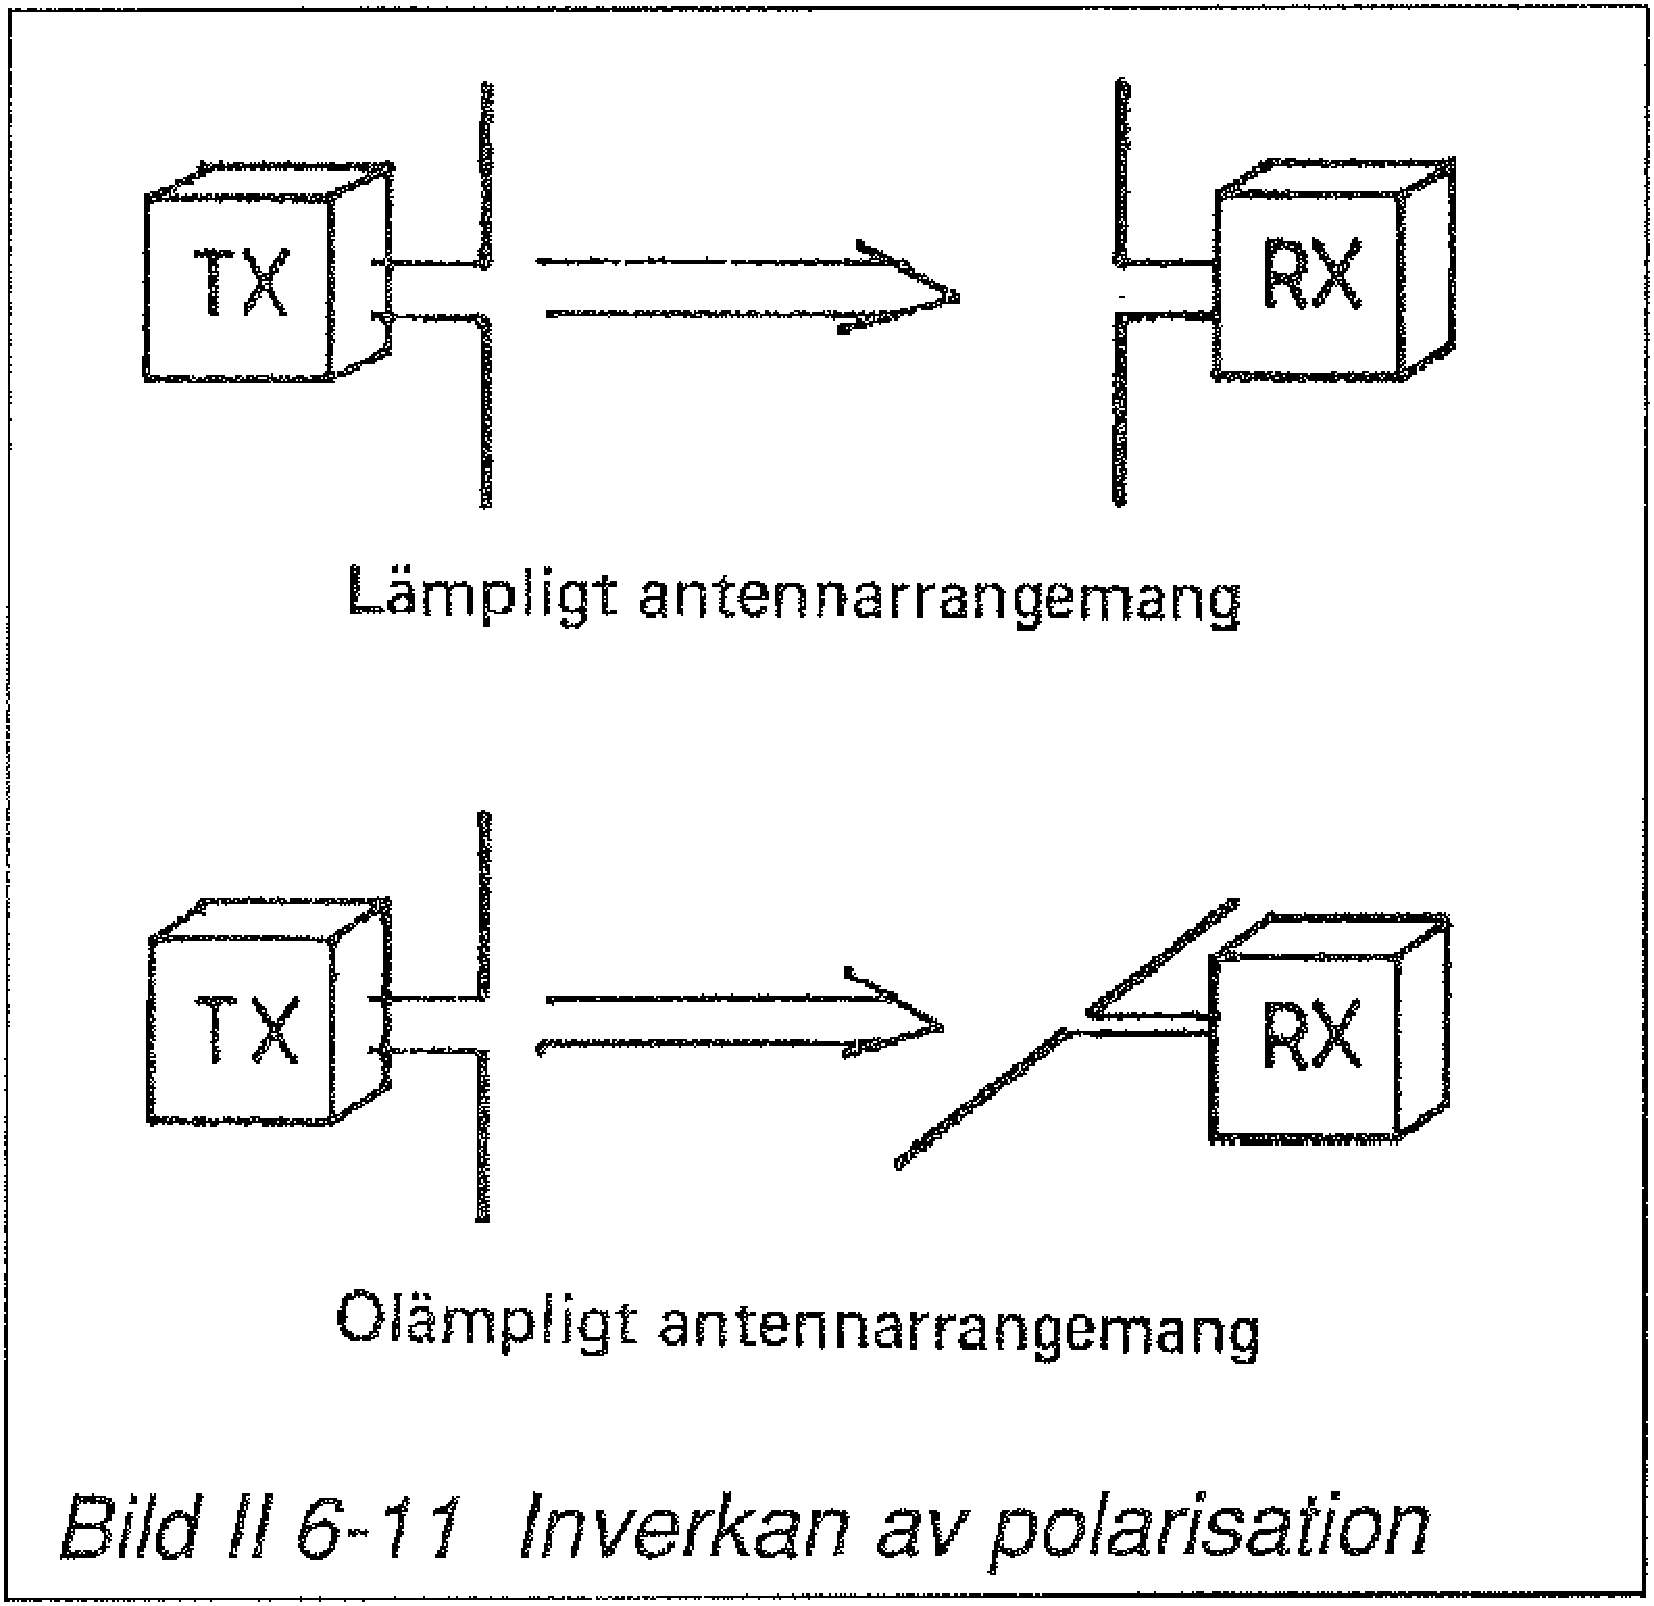
\includegraphics[width=0.5\textwidth]{images/bild_2_6-11}
  \caption{Inverkan av polarisation}
  \label{fig:bildII6-11}
\end{wrapfigure}

I dessa högre frekvensområden tillämpas både horisontell, vertikal och
cirkulär polarisation.

Polarisationsriktningen ändras inte spontant under överföringen så
länge som vågorna inte reflekterats på vägen. Jämför med sändningar
från rymdsatelliter då två program sänds på samma frekvens, men med
olika polarisation. Satelliten får då inte ändra läge i förhållande
till jorden.

För cirkulärt polariserade antenner, där polarisationen vrider sig
omkring utbredningsaxeln, gäller att överföringen är bäst, när
vridningens riktning är lika både i sändar-och mottagarantennen.

Bild \ref{fig:bildII6-11}

